\chapter{Результаты проектирования}

\begin{annotation}
	В данной главе разрабатываются функциональные и пользовательские требования к веб-приложению.
	Проектируется общая архитектура приложения для автоматического когнитивного картирования.
	Описаны этапы обработки данных для автоматического когнитивного картирования.
	Описывается архитектура приложения.
\end{annotation}


% ================ из 2 главы


% \section{Описание этапов обработки данных для когнитивного картирования}

% % \begin{annotation}
% % 	В данном разделе описываются методы обработки данных для автоматического когнитивного
% % 	картирования. Описывается, как можно интерпретировать результат разрабатываемой системы
% % 	и как обработка данных может повлиять на результат вычислений.
% % 	Описываются теоретические принципы работы разрабатываемой системы.
% % \end{annotation}

% Данные в систему могут поступать из разных источников. Так как данные из разных источников
% могут быть в разных форматах, в модулях, в которых производится предобработка данных
% они приводятся к единому виду и нормализуются. После этого собранные данные должны подвергнуться
% анализу. В процессе этого анализа наша система обогащает данные метками или тегами, задает каждому
% объекту вес. Часть меток может браться из первоисточника, если первоисточник предоставляет такие данные.

% Таким образом перед тем, как эксперт может начать работать с данными, они проходят следующие этапы:

% \begin{itemize}
% 	\item скачивание
% 	\item нормализация
% 	\item обогащение
% \end{itemize}

% Так как полученных данных может оказаться слишком много, для работы эксперт может ограничить количество
% концептов различного типа. И уже на их основе разрабатывать карту.

% Под нормализацией данных подразумевается то, что слова в текстах должны быть приведены к единообразному виду.
% Для этого можно использовать стемминг и лемматизацию. Так как данных в системе может быть много, а лемматизация
% на порядок дольше \cite{vallbe2007stemming}, чем стемминг, в данной работе будет исползоваться стемминг.

% \begin{definition}
% Стемминг - это процесс нахождения основы слова для заданного исходного слова.
% Основа слова не обязательно совпадает с морфологическим корнем слова.
% \end{definition}

% \begin{definition}
% Лемматизация - процесс приведения словоформы к лемме — её нормальной (словарной) форме.
% \end{definition}

% Лемматизация требует более строго разбора слова и достаточно требовательна к вычислительным ресурсам.

% =================


\section{Разработка системных, функциональных требований к веб-приложению}
\begin{annotation}
	В данном разделе разрабатываются системные, функциональные и пользовательские требования к
	проектируемому веб-приложению. Выдвигаются требования к масштабируемости приложения,
	к нагрузкам, которые должна выдержать система и скорость отклика и работы системы.
	Выдвигаются требования по возможности расширения данной системы.
\end{annotation}

% В предыдущей работе уже были выдвинуты требования к горизонтальному масштабированию.
% И была достигнута цель в горизонтальном масштабировании при получении данных. Но
% так как все данные хранились и анализировались внутри одной СУБД (PostgreSQL),
% в системе отсутствовало горизонтальное масштабирование при предобработке данных.

% Для того, чтобы достичь этой цели, в данной работе предлагается использовать очереди.
% Так же как и для решения задачи горизонтального масштабирования по обработке данных.

% В системе должна появиться возможность обработки данных из нового источника, а именно,
% с сайта новостей https://lenta.ru.

\section{Архитектура системы}
\begin{annotation}
	В данном разделе рассматривается общая архитектура системы.
	Описывается взаимодействие разных компонент системы между собой.
	А так же взаимодействие системы с пользователем.
	Описываются методы, используемые для обеспечения отказоустойчивости системы.
\end{annotation}

% По сравнению с архитектурой приложения в прошлой работе,
% мы отказываемся от обработки текстов в СУБД PostgreSQL в пользу
% более гибких методов с использованием очередей и Python'а.

% Frontend и Backend API часть приложения не подвергаются большим изменениям.

% % Команда \texorpdfstring необходима, чтобы программа просмотра PDF документов
% % верно отображала текст формул в панели оглавления.
% % При отсутствии команды \texorpdfstring там, где она необходима, LaTeX выводит
% % предупреждение "Token not allowed in a PDF string"

% % \section{Архитектура подсистемы обработки данных}
% % \begin{annotation}
% % 	В данном разделе рассматривается подсистема обработки данных,
% % 	на основе которых будет строиться нечеткая когнитивная карта.
% % 	Проектируется инфраструктура, которая могла бы обеспечить
% % 	исполнение выдвинутых ранее функциональных и системных требований.
% % 	И как будет обеспечиваться отказоустойчивость подсистемы.
% % \end{annotation}

% В подсистеме обработки данных обработка текста будет проводиться не средствами СУБД
% (система управления базами данных), а с помощью обработчиков очередей.
% Это позволит распределить нагрузку и даст большую гибкость в экспериментах и в работе с данными.
% Кроме того, для реализации очередей должен быть использован ассинхронный фреймворк.
% Это позволит повысить производительность обработчиков событий очереди на определенных
% типах задач.

% % \section{Архитектура подсистемы вычисления нечеткой когнитивной карты}
% % \begin{annotation}
% % 	В данном разделе рассматривается подсистема вычисления нечеткой когнитивной карты.
% % 	Описывается, как будет происходить пересчет значений концептов карты.
% % 	Описывается, аппаратные компоненты могли бы повысить производительность подсистемы.
% % 	Рассматривается возможность системы к распараллеливанию вычислений.
% % \end{annotation}

% В подсистему вычисления нечеткой когнитивной карты добавлены методы
% для расчета карты с помощью TTR NFCM.

% \begin{figure}
% 	\begin{center}
% 		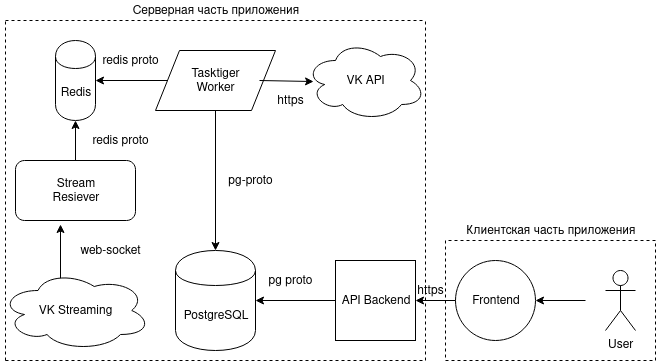
\includegraphics[width=.5\columnwidth]{./img/architecture_old.png}%
% 		\caption{Диаграмма потоков данных предыдущей версии архитектуры}%
% 		\label{pic:architecture_old}%

% 		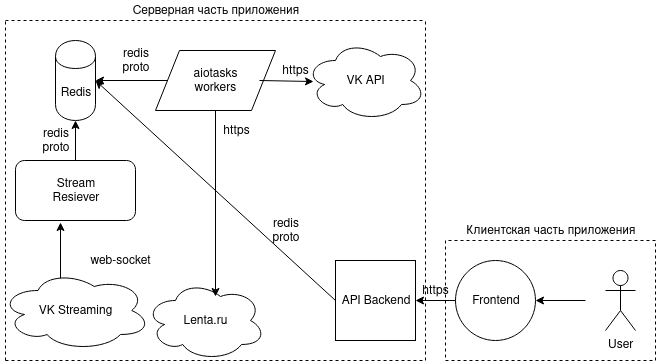
\includegraphics[width=.5\columnwidth]{./img/architecture_new.png}%
% 		\caption{Диаграмма потоков данных текущей версии архитектуры}%
% 		\label{pic:architecture_new}%
% 	\end{center}
% \end{figure}


% По сравнению с прошлой версией \ref{pic:architecture_old},
% текущая архитектура \ref{pic:architecture_new} имеет меньшее количество
% внутренних компонентов, но тем не менее не теряет способность к масштабированию.
% А то, что в текущей версии меньше внутренних компонентов позволяет упростить ее
% эксплуатацию и увеличивает отказоустойчивость системы, потому что в предыдущей версии
% системы было больше возможных точек отказа. Кроме того, обработчики очередей
% проще масштабировать, чем реляционную СУБД. Потому что для обработчиков очередей узкое
% место ~- это Redis. А nosql базы данных, в данном случае redis, горизонтально масштабировать проще \cite{carlson2013redis},
% чем реляционные.


\section{Выводы}
Было спроектирована система для автоматического когнитивного картирования с
использованием нейросетевых методов с возможностью расширения количества
источников, из которых берутся исходные данные.

Спроектированная система содержит следующие подсистемы:
\begin{itemize}
	\item Подсистема обработки данных. С возможностью добавления источников данных.
	\item Подсистема вычисления когнитивной карты. С возможностью распараллеливания вычислений.
	\item Backend REST API. С возможностью горизонтального масштабирования.
	\item Frontend.
\end{itemize}
